%%%%%%%%%%%%%%%%%%%% author.tex %%%%%%%%%%%%%%%%%%%%%%%%%%%%%%%%%%%
%
% sample root file for your "contribution" to a contributed volume
%
% Use this file as a template for your own input.
%
%%%%%%%%%%%%%%%% Springer %%%%%%%%%%%%%%%%%%%%%%%%%%%%%%%%%%


% RECOMMENDED %%%%%%%%%%%%%%%%%%%%%%%%%%%%%%%%%%%%%%%%%%%%%%%%%%%
\documentclass[graybox]{svmult}

% choose options for [] as required from the list
% in the Reference Guide

\usepackage{mathptmx}       % selects Times Roman as basic font
\usepackage{helvet}         % selects Helvetica as sans-serif font
\usepackage{courier}        % selects Courier as typewriter font
\usepackage{type1cm}        % activate if the above 3 fonts are
                            % not available on your system
%
\usepackage{makeidx}         % allows index generation
\usepackage{graphicx}        % standard LaTeX graphics tool
                             % when including figure files
\usepackage{multicol}        % used for the two-column index
\usepackage[bottom]{footmisc}% places footnotes at page bottom

% see the list of further useful packages
% in the Reference Guide

\makeindex             % used for the subject index
                       % please use the style svind.ist with
                       % your makeindex program

%%%%%%%%%%%%%%%%%%%%%%%%%%%%%%%%%%%%%%%%%%%%%%%%%%%%%%%%%%%%%%%%%%%%%%%%%%%%%%%%%%%%%%%%%


% Additional Packages %%%%%%%%%%%%%%%%%%%%%%%%%%%%%%%%%%%%%%%%%%%%%%%%%%%
\usepackage[version=4]{mhchem}
\usepackage[capitalize]{cleveref}
\usepackage[usenames,dvipsnames]{xcolor}
\usepackage{bm}
\usepackage[caption=false]{subfig}
%\usepackage{textcomp}
\usepackage{tikz}
\usetikzlibrary{decorations.markings}
\usetikzlibrary{shapes.misc,shapes.geometric,arrows,positioning,automata, patterns}


% ####################################################################################
% Bibliography definitions
% ####################################################################################
%\usepackage[
%    style=spphys,
    %sorting=none,
    %biblabel=brackets,
    %articletitle=true,
    %giveninits=true,
    %maxbibnames=5,
    %url=false,
    %doi=false,
    %isbn=false,
    %backend=biber
%]{bibtex} % Load the package with some options.
%\AtEveryBibitem{%
%    \clearlist{language}%
%    \clearfield{note}%
%} % delete some entries that are note needed in the bibliographyy
%\addbibresource{mylit.bib} % add bibtex file



% Additional Definitions %%%%%%%%%%%%%%%%%%%%%%%%%%%%%%%%%%%%%%%%%%%%%%%%%%%
\newcommand{\matr}[1]{\bm{\mathit{#1}}}
\newcommand{\beq}{\begin{equation}}
\newcommand{\eeq}{\end{equation}}


\begin{document}

\title*{KKRnano: Quantum Description of Skyrmions in Chiral B20 Magnets}
% Use \titlerunning{Short Title} for an abbreviated version of
% your contribution title if the original one is too long
\author{Marcel Bornemann \and Paul F. Baumeister \and Rudolf Zeller \and Stefan Bl\"ugel}
% Use \authorrunning{Short Title} for an abbreviated version of
% your contribution title if the original one is too long
\institute{Marcel Bornemann \at Peter Gr\"unberg Institute and (PGI-1) and Institute for Advanced Simulation (IAS-1), Forschungszentrum J\"ulich, 52425 J\"ulich,
Germany \& RWTH Aachen University, 52056 Aachen, Germany, \email{m.bornemann@fz-juelich.de}
\and Paul F. Baumeister \at  J\"ulich Supercomputing Centre, Forschungszentrum J\"ulich, 52425 J\"ulich,
Germany, \email{p.baumeister@fz-juelich.de}
\and Rudolf Zeller \at Institute for Advanced Simulation (IAS-1), Forschungszentrum J\"ulich, 52425 J\"ulich,
Germany, \email{ru.zeller@fz-juelich.de}
\and Stefan Bl\"ugel \at Peter Gr\"unberg Institute and (PGI-1) and Institute for Advanced Simulation (IAS-1),
Forschungszentrum J\"ulich, 52425 J\"ulich,
Germany, \email{s.bluegel@fz-juelich.de}}
%
% Use the package "url.sty" to avoid
% problems with special characters
% used in your e-mail or web address
%
\maketitle
\abstract{
We present the latest version of the linear-scaling electronic structure code KKRnano, in which
an enhanced 
Korringa-Kohn-Rostoker (KKR) scheme is utilized to perform Density Functional Theory (DFT) calculations.
The code allows us to treat system sizes of up to several thousands of atoms per unit cell and to
simulate a non-collinear alignment of atomic spins.
This capability is used to investigate nanometer-sized magnetic textures in the germanide B20-\ce{MnGe},
a material that is potentially going to play an important role in future spintronic devices.
A performance analysis of KKRnano on Hazel Hen emphasizes the good scaling behaviour with increasing
system size and demonstrates the extensive integration of highly optimized libraries.
}

\section{Introduction}
\label{sec:intro}
We have developed a unique electronic structure code, 
KKRnano \cite{zeller_towards_2008,thiess_massively_2012,bornemann_large-scale_nodate},
specifically designed for petaFLOP computing. Our method scales linearly
with the number of atoms, so that we can realize system sizes of up to 
half a million atoms in a unit cell if necessary.
Recently, we implemented a relativistic generalization of our algorithm 
enabling us to calculate complex non-collinear magnetic structures, such as skyrmions,
in real space. Skyrmions are two-dimensional magnetization solitons, i.e., two-dimensional
magnetic structures localized in space, topologically protected by a non-trivial
magnetization texture, which has particle-like properties. 
The focus of our work is on the germanide \ce{MnGe} that is particularly
interesting among the chiral magnetic B20 compounds, as it exhibits a three-dimensional magnetic structure
that is not yet understood (see preliminary results
\cite{tanigaki_real-space_2015,rybakov_new_2016,bornemann_investigation_2017,bornemann_large-scale_2018}).

This report is structured as follows:
In \cref{sec:methods_algorithms} we give a brief introduction on the Korringa-Kohn-Rostoker (KKR) 
method and explain how
linear scaling is achieved.
Our results on B20-\ce{MnGe} are presented in \cref{sec:mnge}.
In \cref{sec:par_scheme} and \cref{sec:performance} the focus is on code-specific issues. 
The parallelization scheme of KKRnano
is described in detail and a performance analysis of our code on Hazel Hen is conducted.


\section{Numerical Methods and Algorithms}
\label{sec:methods_algorithms}
%\rule{\textwidth}{0.4pt}\\
%\textit{Describe the numerical methods and algorithms that you are planning to use, improve, or develop.}\\
 
%\textit{(1 to 2 pages)}
%\bigskip

Contrary to other Density Functional Theory (DFT) codes, which determine the Kohn-Sham orbitals by solving
the Kohn-Sham differential wave equation, in KKRnano the Green function for the Kohn-Sham
equation is obtained by solving an integral equation in real space. In this so called Korringa-Kohn-Rostoker
(KKR) scheme, space is divided
into non-overlapping cells around the atoms, and the calculations are separated into single-cell parts
where only the potential within the individual cell enters, and a large complex linear matrix equation for 
the matrix elements $G_{LL}^{nn'} (\epsilon)$ of the Green function $G(r, r , \epsilon)$:
\begin{equation}
	G_{LL'}^{nn'} (\epsilon) = G_{LL'}^{r,nn'} (\epsilon) + \sum_{n''} \sum_{L''}
	G_{LL''}^{r,nn''} (\epsilon) \sum_{L'''} \Delta t_{L'' L'''}^{n''} (\epsilon)
	G_{L'''L'}^{n''n'} (\epsilon)
	\label{eq:dyson_eq}
\end{equation}
In the following we refer to $\Delta t_{L'' L'''}^{n''} (\epsilon)$ as the $\Delta t$-matrices and
$G_{LL''}^{r,nn''} (\epsilon)$ as the reference Green functions. We refer the reader to the existing
literature for more details \cite{zeller_towards_2008}.
The problem given in \cref{eq:dyson_eq} is identical to solving a complex linear matrix equation of the form
\begin{equation}
	\label{eq:axb}
	\matr{A} \vec{x} = \vec{b}.
\end{equation}
As is well known, this problem scales as $O(N^3)$, where $N$ denotes the dimension of the $N \times N$
matrix $\matr{A}$. Standard solving schemes therefore severely limit the system size that can
be calculated.
However, by choosing a reference system of repulsive potentials,
$\matr{A}$ can be made sparse and this can be exploited
by using customized iterative algorithms for solving linear sparse matrix equations.
Our method uses the transpose-free quasi-minimal-residual (TFQMR) algorithm \cite{freund_qmr:_1991}
which enables us to achieve $O(N^2)$ scaling. 
Convergence of the TFQMR iterations is achieved by working in the complex energy plane. Both concepts,
the repulsive reference system and application of complex energy, were
introduced by us into the KKR method \cite{zeller_application_1982,zeller_theory_1995}
and are used worldwide for many years. 
By truncating inter-atomic interactions above a certain distance, an $O(N)$ scaling 
behavior can be realized, and this feature should be used in any calculation involving more than 1000 atoms.
In most applications the TFQMR solver accounts for the major part of the computational work.

For super-large-scale calculations (above 100,000 atoms) the electrostatics solver begins
to require an amount of computing resources that is not negligible anymore \cite{brommel_juqueen_2017}. 
The electrostatic problem is given in terms of a Poisson equation that connects electric field and potential. 
Solving this equation scales quadratically with system size, a drawback which will be removed in the future.

\section{Complex Magnetic Textures in B20-\ce{MnGe}}
\label{sec:mnge}

B20-\ce{MnGe} was identified as a good candidate material to be investigated with the new
version of KKRnano which now contains the feature of non-collinear magnetism and spin-orbit coupling.
In a recent study \cite{tanigaki_real-space_2015}, it was 
found by transmission electron microscopy that 3D magnetic
objects exist in B20-\ce{MnGe}. The authors of \cite{tanigaki_real-space_2015}
came to the conclusion that their data indicates a
cubic lattice of skyrmionic hedgehogs
and anti-hedgehogs (see \cref{fig:mnge_3q}) 
with a lattice constant of about 3-6 nm.
The singularity at the center of the texture exists only in the micromagnetic description since the
atomic magnetic moment of the atom, which is located at the center,
remains finite \cite{feldtkeller_continuous_2017}.
\begin{figure}[htb]
	\subfloat[]{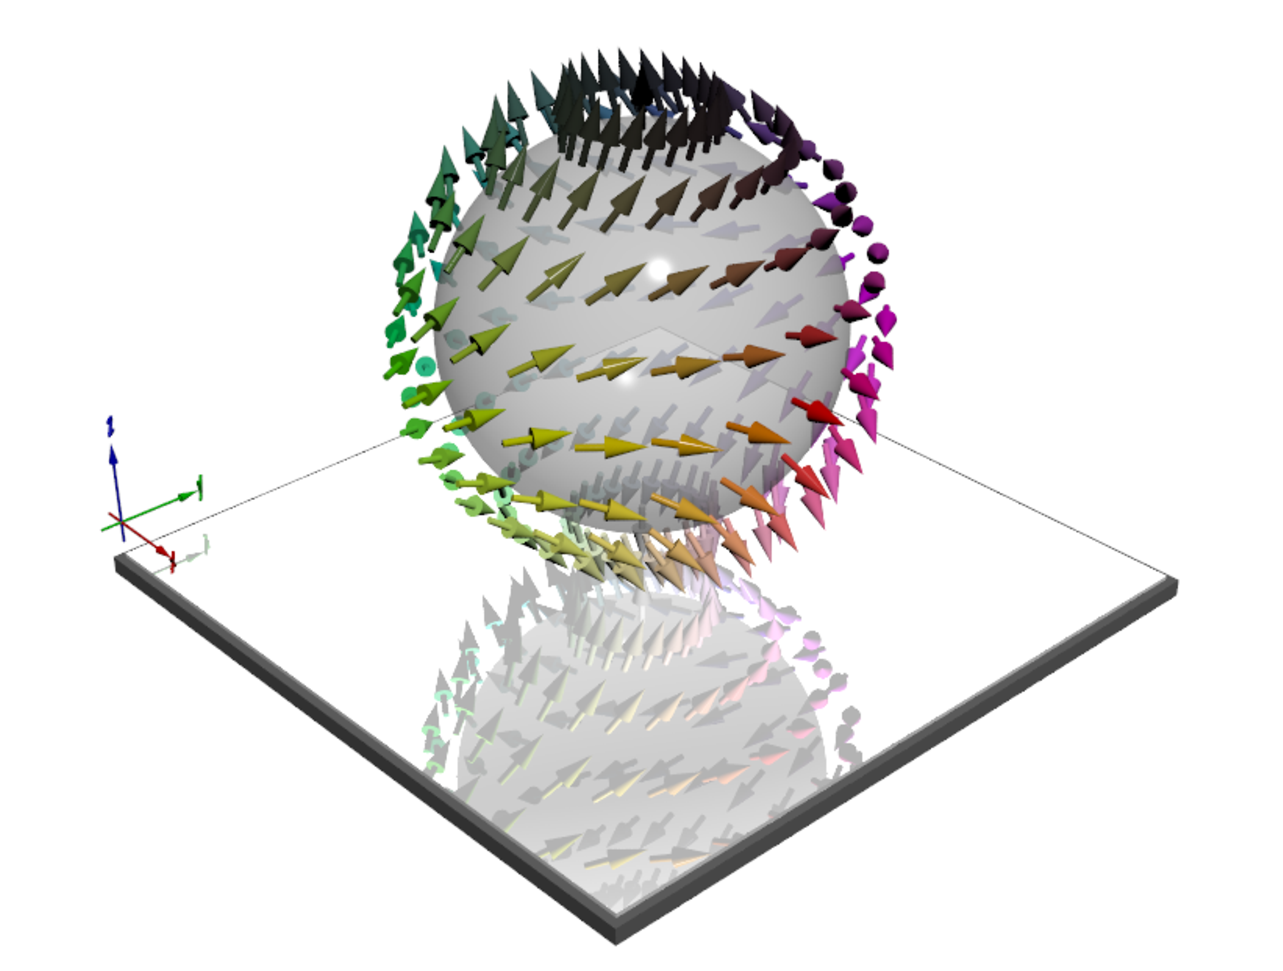
\includegraphics[width=.50\textwidth]{Figures/antihedgehog.eps}\label{fig:mnge_3q}}
	\hfill
	\subfloat[]{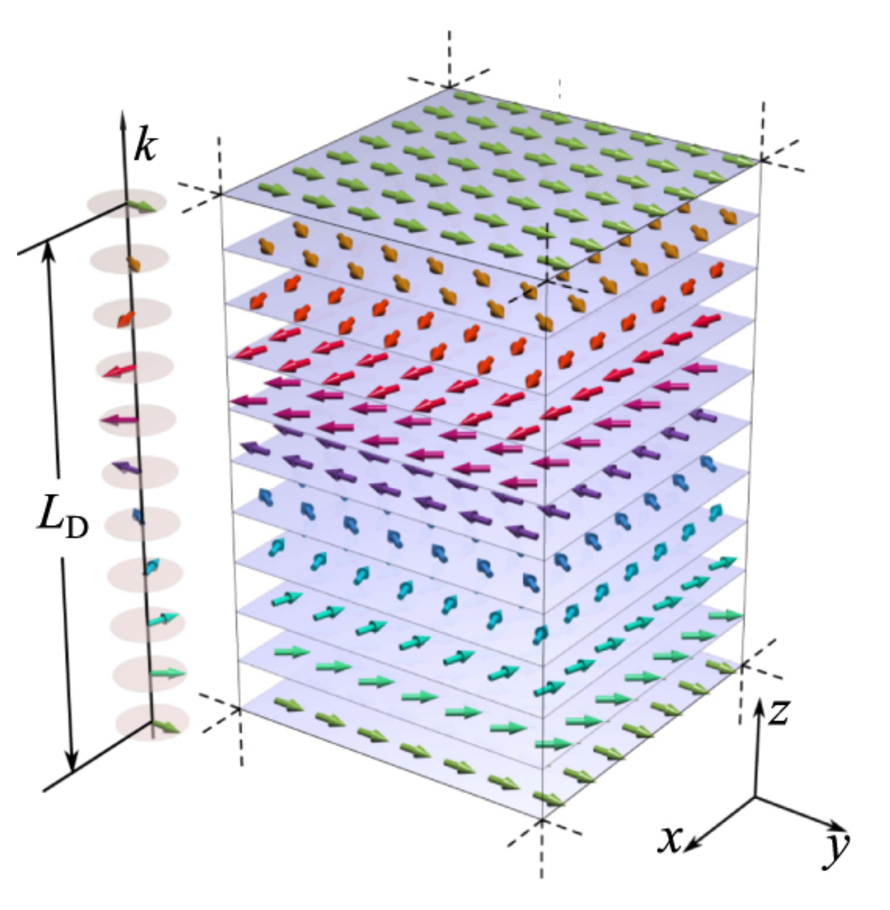
\includegraphics[width=.50\textwidth]{Figures/helicalspiral.eps}\label{fig:mnge_spiral}}
	\hfill
 \caption{Magnetic textures that are found experimentally in B20-\ce{MnGe}: (a) 
	Magnetic anti-hedgehog texture that is wrapped around a singularity at the center.
	Published with kind permission of © Nikolai Kiselev 2018. All Rights Reserved. (b) Helical
	spin spiral that propagates in (001) direction. Reprinted from \cite{rybakov_new_2016} and
	licensed under CC BY 3.0.}
\end{figure}
Findings by Kanazawa \textit{et al.} suggest that the lattice is set up by a superposition of three orthogonal
helical structures, also referred to as 3Q state \cite{kanazawa_noncentrosymmetric_2017}. 
Here, the local magnetization is determined by the provision
\beq
\label{eq:3q_formula}
\vec{M}(\vec{r}) =
\begin{pmatrix}
	\sin{qy} + \cos{qz} \\
	\sin{qz} + \cos{qx} \\
	\sin{qx} + \cos{qy}
\end{pmatrix},
\eeq
where $q=\frac{2\pi}{\lambda}$ is the wavenumber given in terms of the helical wavelength $\lambda$ and
$x$, $y$ and $z$ are the spatial coordinates within the unit cell.
Note, that $\vec{M}(\vec{r})$ is not normalized.
In contrast to other systems exhibiting a
similar magnetic phase, the rather short helical wavelength in B20-\ce{MnGe} allows one to perform
Density Functional Theory (DFT) 
calculations with KKRnano.
B20-\ce{MnGe} is currently the subject of extensive
investigation
\cite{kanazawa_large_2011,kanazawa_possible_2012,grigoriev_chiral_2013,tanigaki_real-space_2015,martin_magnetic_2016}.
This is mainly inspired by the discovery of skyrmions as small information-carrying particles
that could potentially be used in spintronic devices \cite{fert_magnetic_2017}.
However, no large-scale DFT calculation seems to have been performed, yet.
At present there is a lack of a convincing explanation
of what is observed in experiment. Research in the framework of micromagnetic models identified both
magnetic frustration (RKKY interaction) as well as spin-orbit coupling induced Dzyaloshinskii-Moriya (DM)
interaction as potentially crucial to a better
understanding \cite{altynbaev_hidden_2016,koretsune_control_2015}. 
While the 3Q state certainly constitutes the most interesting non-trivial magnetic texture 
in B20-\ce{MnGe}, there are also reports that the magnetic ground state in this system is
actually a helical spiral (see \cref{fig:mnge_spiral}) \cite{yaouanc_magnetic_2017} which was observed up
to a temperature of 170 K \cite{makarova_neutron_2012}.
These two observations are clearly contradictory and it has not yet been explained how
both can coexist within the same material.
The helical spin spiral in B20-\ce{MnGe} forms along the (001) direction and therefore the magnetization
is described by the relation
\beq
\label{eq:1q_spiral}
\vec{M}(\vec{r}) =
\begin{pmatrix}
	 \cos{qz} \\
	-\sin{qz}  \\
	0
\end{pmatrix}
.
\eeq
In the following, we refer to this as the 1Q state.

We commence our investigations by considering a 6x6x6 B20-\ce{MnGe} supercell (1728 atoms), where we use PBEsol 
as exchange-correlation functional
and include only a single k-point, i.e., the $\Gamma$-point.
In this initial comparison of ferromagnetic (FM), 1Q and 3Q state the respective states are imposed on
the system by forcing the atomic exchange-correlation B-fields
to point into specific directions. 
For the equilibrium lattice constant
$a=4.80$ \AA, the ferromagnet is the state with the lowest total energy.
As this contradicts experimental observations, we take into consideration that
in experiment the crystal structure might inadvertently differ from the ideal structure.
Such discrepancies can for instance be caused by strain that 
originates from the manufacturing process of the sample.
Therefore, it is reasonable to check whether a material's magnetic properties change, when the
lattice constant is varied.
\begin{figure}[htb]
  \centering
   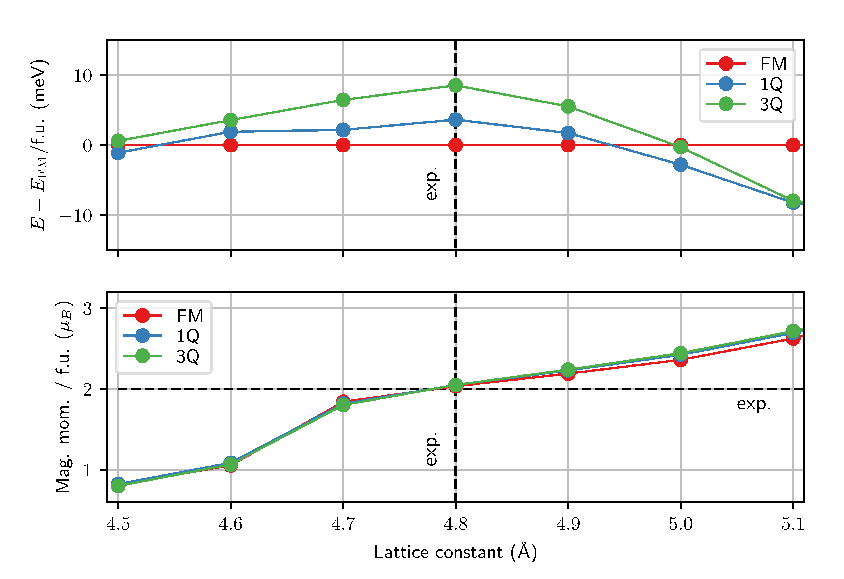
\includegraphics[width=1.00\textwidth]{Figures/MnGe_ferro_1q.eps}
	\caption{Comparison of Ferromagnetic (FM), helical spiral (1Q) and hedgehog lattice (3Q) 
	state with KKRnano.
	Top: Difference of total energies with the FM state as reference state for different
	lattice constants. The experimental lattice constant is $a=4.80$ \AA. 1Q and 3Q state
	are energetically preferable for $a > 5.0$ \AA.
	Bottom: Magnetic moment per \ce{Mn} atom increases with lattice constant.
	High-spin/Low-spin transition is clearly visible between $a=4.60$ and $a=4.70$ \AA.
	Experimentally, the magnetic moment is measured to be $\approx 2 \mu_B$.
	Published with kind permission of © Marcel Bornemann 2018. All Rights Reserved.}
\label{fig:MnGe_kkrnano_comparison}
\end{figure}
Such a variation is performed in the upper part of \cref{fig:MnGe_kkrnano_comparison}, where
the total energy is evaluated for FM, 1Q and 3Q state.
Clearly, neither the 1Q nor the 3Q state constitutes the ground state,
when the experimental lattice constant is assumed.
Yet, by increasing or decreasing the lattice constant the energetic difference can be made
smaller.
We focus on an increase of the lattice constant rather than a decrease since 
the system goes into the low-spin state below $a=4.65$ \AA \, \cite{rosler_ab_2012} and according to experiment
the non-trivial textures
exist in the high-spin regime.
A crucial transition point is found around $a=5.0$ \AA,
where by imposing the 1Q or 3Q state the energy can be made smaller than for the ferromagnetic state.
In general, for $a>5.0$ \AA \, both helical states are favored over the ferromagnetic one.
Obviously, an artificial increase of the lattice constant by
$0.2$ \AA \, ($\approx 4 \%$) or more is fairly large.
However, probes in experiment are seldom if ever perfectly clean and
impurities in the sample need to be considered as a source of error in the
final analysis. One potential
effect of impurities is chemical pressure that causes a spatial expansion of the
lattice structure.
An example of the possible effects of positive chemical pressure
can be found in \ce{Co}-doped B20-\ce{FeGe} \cite{stolt_chemical_2018}. 
Here, it was experimentally observed
that doping can increase the melting temperature and change the magnetic properties of a B20 alloy.
In the lower part of \cref{fig:MnGe_kkrnano_comparison}, the evolution of the magnetic moment
with varying lattice constant is tracked.
The resulting magnetic moment for the experimental lattice constant nicely falls 
on top of the magnetic moment of approximately $2 \mu_{B}$/f.u. 
which is reported by experimentalists \cite{yaouanc_magnetic_2017}.
Furthermore, the high-spin/low-spin transition is recognizable between $a=4.60$ and $a=4.70$ \AA.
It can also be observed that the magnetic moment increases, when the lattice constant is increased.
This is a common behaviour which is often observed in metallic systems.
For larger lattice constants the magnetic moments of the three different
magnetic textures differ more than for the smaller lattice constants.
This might be connected to the observation of the differences in the total energy.

We continue our investigation of B20-\ce{MnGe} by studying the influence of spin-orbit
coupling (SOC) enhancement on the magnetic energy landscape.
An advantage of the way SOC is implemented in KKRnano is that
its contribution is added to the scalar-relativistic
potential in a perturbation-like manner. This allows to scale its strength and make it
artificially stronger.
\begin{figure}[htb]
	\sidecaption
	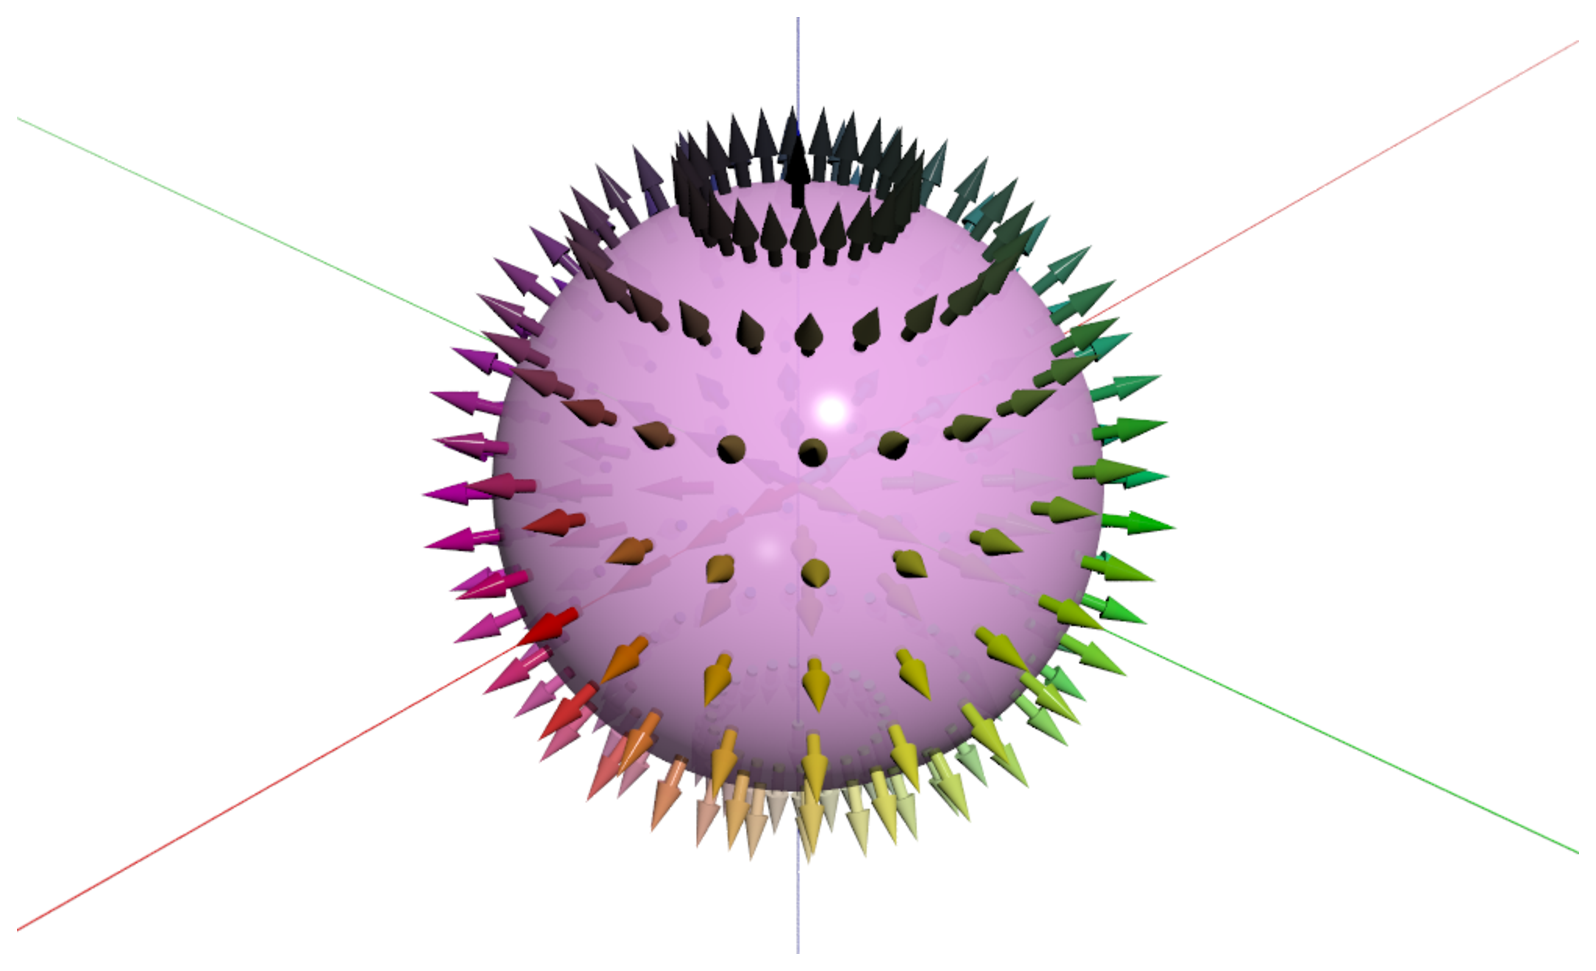
\includegraphics[width=0.55\textwidth]{Figures/blochpoint.eps}
	\caption{Illustration of a Bloch point in real space with all magnetic moments
	pointing out of the center of the Bloch sphere.
	We use the same magnetic configuration but invert the spin direction so that all moments point
	into the center. Published with kind permission of © Nikolai Kiselev 2018. All Rights Reserved.
	}
	\label{fig:mnge_blochpoint}
\end{figure}
In this context we perform a comparison of the Bloch point (BP) state 
and the ferromagnetic (FM) state.
The BP texture is defined by means of the four spherical parameters $\phi$, $\theta$, 
$\Phi$ and $\Theta$.
$\phi$ and $\theta$ designate the position of an \textbf{individual atom} in the unit cell
which is described by the radius $r$ and the common polar and azimuthal angle
\beq
\phi = \arctan{\left(y/x\right)}
\eeq
and
\beq
\theta = \arccos{\left( \frac{z}{\sqrt{x^2+y^2+z^2}} \right)}.
\eeq
The BP texture does not depend on $r$ and we can therefore neglect it in the following.
Usually, the atomic positions are given in the Cartesian coordinates $x,y$ and $z$.
In the definition above, we define the origin of the coordinate system, i.e., the tuple $(x=0, \, y=0, \, z=0)$,
to be at the center of the unit cell.
In this frame of reference, all atoms that lay in an x-y-plane that intersects with the center
are described by $\theta=\pi/2$.
The orientation of the \textbf{individual atomic magnetic moments} for a BP texture is then defined 
by the polar angle
\beq
\Phi = \phi + \phi_{1}
\eeq
and the azimuthal angle
\beq
\Theta = 2 \arctan{\left(\cot{\frac{\theta}{2}} \right)},
\eeq
where the angles designating the atomic position enter as arguments. $\phi_{1}$ is a phase factor.
An illustration of a BP is given in \cref{fig:mnge_blochpoint}. Note, that in contrast to
that illustration we conduct our investigation for a BP with $\phi_{1}=\pi$, where magnetic moments
are inverted, i.e., all moments point into instead of out of the center.
\\
For our calculations we
again use a 6x6x6 supercell but this time with a 2x2x2 k-point-mesh and LDA as
exchange-correlation functional. Here, we choose LDA because it has been used extensively in all KKR codes
in the past and 
we want to eliminate the possibility of numerical problems that could occur when SOC is artificially enhanced.
The magnetic moments are allowed to relax during the convergence process.
This leads to a small canting of the moments which is a known effect in
B20 materials \cite{chizhikov_multishell_2013}.
\begin{figure}[!htb]
  \centering
   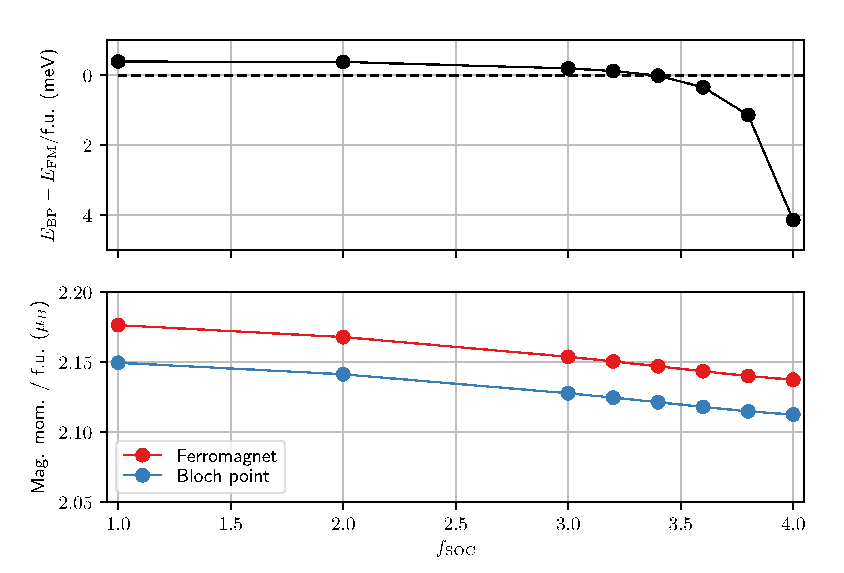
\includegraphics[width=1.00\textwidth]{Figures/MnGe_ferro_bp.eps}
	\caption{Effect of increased SOC on B20-\ce{MnGe} in a 6x6x6 supercell.
	Top: Total energy difference between (relaxed) Bloch point and (relaxed) ferromagnet.
	Bottom: Magnetic moment of ferromagnet and Bloch point state.
	Published with kind permission of © Marcel Bornemann 2018. All Rights Reserved.}
\label{fig:MnGe_kkrnano_comparison_bp}
\end{figure}
A series of calculations is conducted ranging from the physical value of the SOC 
to
an enhancement of it by a
factor of $f_{\text{SOC}}=4.0$ (see \cref{fig:MnGe_kkrnano_comparison_bp}).
As could be expected from the investigation of 1Q and 3Q state before,
the BP state is energetically not preferred over the FM state for a small
scaling of SOC.
However, when SOC is scaled further up to $f_{\text{SOC}}=3.5$,
both states are energetically more or less equivalent.
Above $f_{\text{SOC}}=3.5$ the BP state is clearly preferred over the FM state with
an energy difference of up to 4 meV/f.u.
Within the parameter range that we checked in this study,
the most beneficial scaling value for the BP is found to be $f_{\text{SOC}}=4.0$.
The effect of SOC scaling on the magnetic moment can be deemed negligible. Over the whole
range it decreases by 0.07 $\mu_{B}$ for each of the two states
(see again \cref{fig:MnGe_kkrnano_comparison_bp}).
It would be interesting to check whether a global minimum of $E_{\text{BP}}-E_{\text{FM}}$ can
be found for $f_{\text{SOC}} > 4.0$. This would hint to an optimal
scaling at which also other non-collinear magnetic textures, e.g., 1Q spin spiral or
3Q hedgehog lattice, can possibly be stabilized.
However, this is not possible as our method becomes increasingly numerically unstable for 
such strong scaling factors, i.e., the total energy does not converge anymore.
The reason for this is currently under investigation.

%\begin{figure}
%	\floatbox[{\capbeside\thisfloatsetup{capbesideposition={right,top}}}]{figure}[\FBwidth]
%{\caption{Illustration of a Bloch point with all magnetic moments pointing out of the center of the Bloch sphere.
%	We use the same magnetic configuration but invert the spin direction so that all moments point
%	into the center. Figure provided by Nikolai Kiselev.}\label{fig:blochpoint}}
%{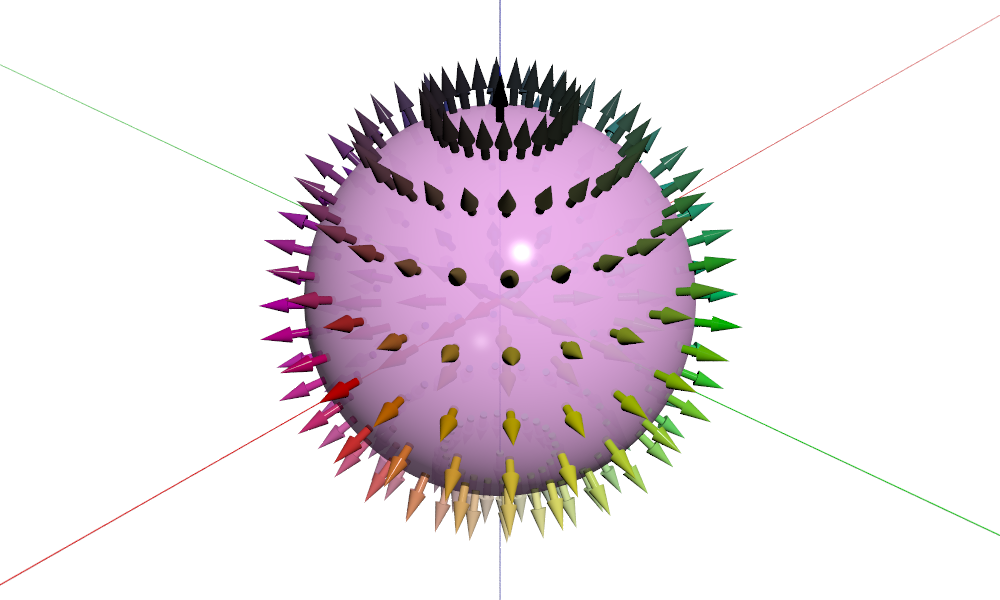
\includegraphics[width=0.6\textwidth]{Figures/blochpoint.png}}
%\end{figure}
%\begin{figure}[htb]
%	\sidecaption
%	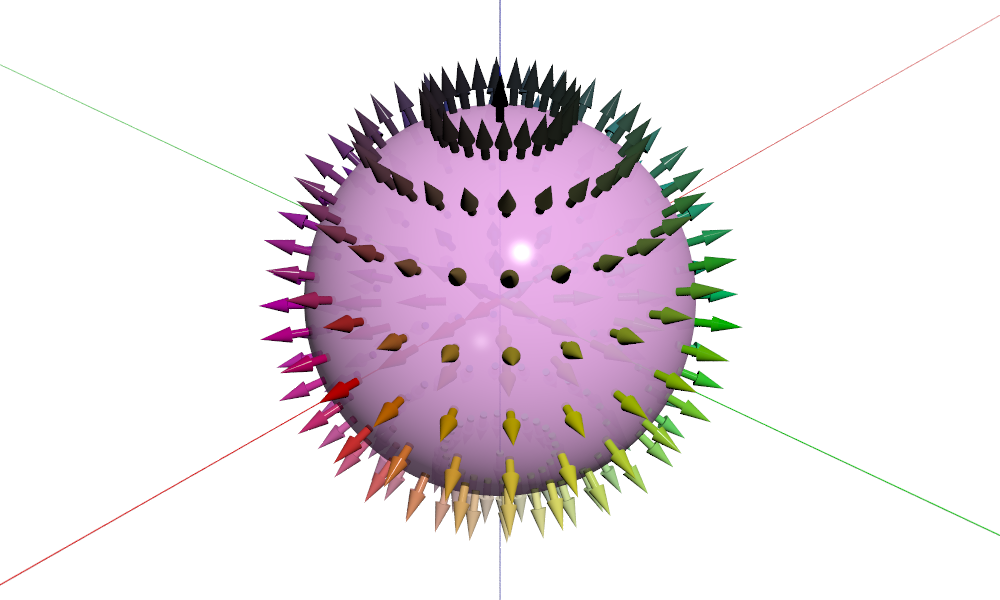
\includegraphics[width=0.55\textwidth]{Figures/blochpoint.png}
%	\caption{Illustration of a Bloch point with all magnetic moments pointing out of
%	the center of the Bloch sphere.
%	We use the same magnetic configuration but invert the spin direction so that all moments point
%	into the center. Figure provided by Nikolai Kiselev.}
%	\label{fig:blochpoint}
%\end{figure}
%On Hazel Hen we perform a comparison of the magnetic Bloch point (BP) (see \cref{fig:blochpoint}) 
%state and the familiar ferromagnetic (FM) state
%with the same supercell size of 6x6x6 as before but with a denser k-point-mesh of 2x2x2 points.
%As exchange-correlation functional we choose LDA and keep the lattice constant fixed to $a=4.80$ \AA.
%We allow the magnetic moments to relax during the convergence process.
%This leads to a small canting of the moments which is a known effect in
%B20 materials \cite{chizhikov_multishell_2013}.
%A series of calculations is conducted ranging from an SOC that is not altered, i.e. $f_{\text{SOC}}=1.0$ to
%an enhancement of the SOC potential by a
%factor of $f_{\text{SOC}}=4.0$ (see \cref{fig:MnGe_ferro_bp_socscale}).
%\begin{figure}[htb]
%\begin{center}
% 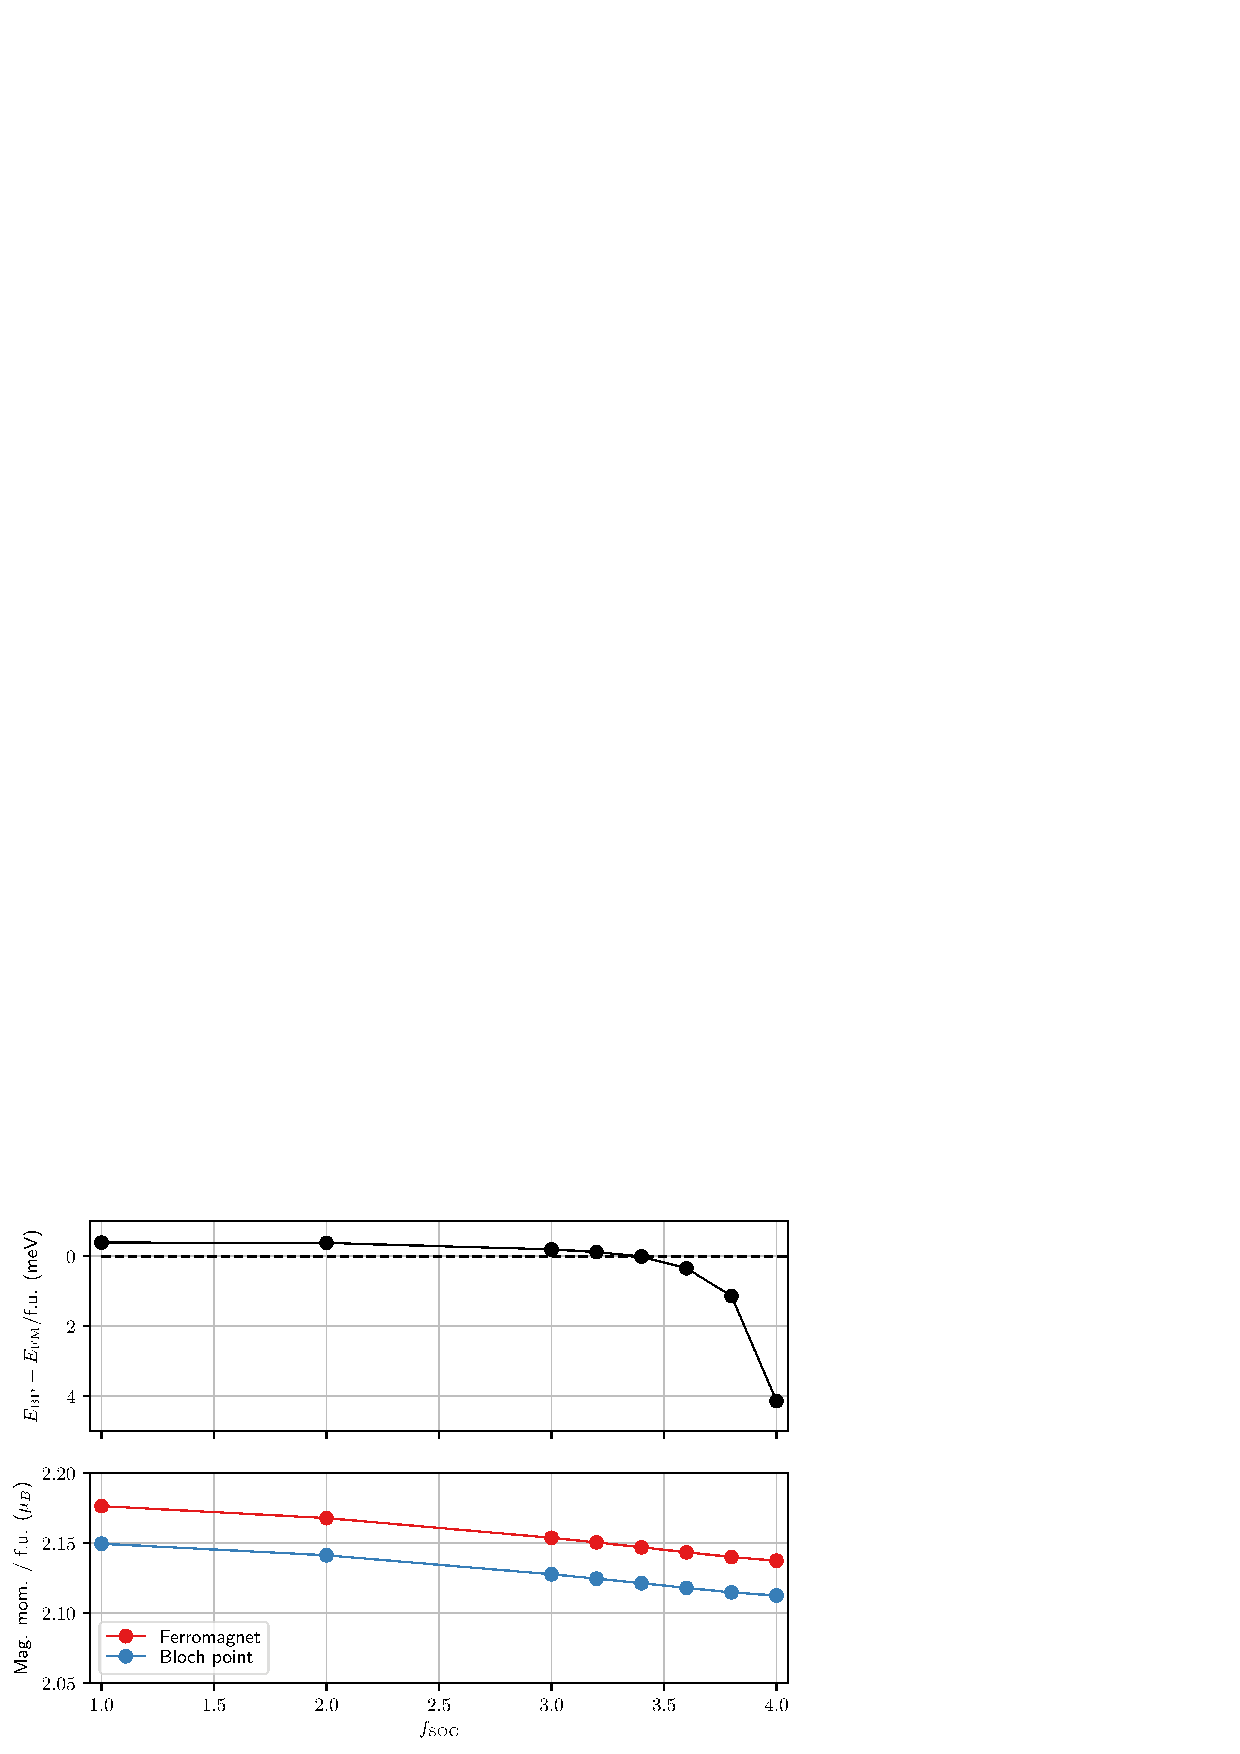
\includegraphics[width=\textwidth]{Figures/kkrnano_MnGe_ferro_bp_socscale/MnGe_ferro_bp.pdf}
%\end{center}
%\caption{Effect of increased SOC on B20-\ce{MnGe} in a 6x6x6 supercell.
%	Top: Total energy difference between (relaxed) Bloch point and ferromagnet per formula unit.
%	Bottom: Magnetic moment per formula unit of ferromagnet and Bloch point state.
%	}
%\label{fig:MnGe_ferro_bp_socscale}
%\end{figure}
%As can be expected from the comparison of non-trivial magnetic textures 
%in \cref{fig:MnGe_ferro_1q}, where $f_{\text{SOC}}=1.0$, 
%the BP state is energetically not preferred over the FM state for a small
%enhancement of SOC.
%When SOC is increased by $f_{\text{SOC}}=3.5$,
%both states are energetically more or less equivalent.
%For $f_{\text{SOC}} \geq 3.5$ KKRnano clearly prefers the BP state over the FM state with
%an energy difference of up to 4 meV/f.u.
%The most beneficial scaling value is found to be $f_{\text{SOC}}=4.0$.
%The effect of SOC scaling on the magnetic moment can be deemed negligible. Over the whole
%range it decreases by 0.07 $\mu_{B}$ for each of the two states.
%It would be interesting to check whether a global minimum of $E_{\text{BP}}-E_{\text{FM}}$ can
%be found for $f_{\text{SOC}} > 4.0$. This would hint to an optimal
%scaling at which also other non-collinear magnetic textures, e.g. 1Q spin spiral or
%3Q hedgehog lattice, can possibly be stabilized.
%However, this is not possible as our method becomes increasingly numerically unstable for 
%such strong scaling factors, i.e. the total energy does not converge anymore.
%The reason for this is currently under investigation.

\section{Parallelization Scheme of KKRnano}
\label{sec:par_scheme}
In order to use the full potential of modern supercomputers,
KKRnano features both MPI and OpenMP parallelization. The parallelization concept is sketched in
\cref{fig:kkrnano_parallel}.
There are three MPI levels to parallelize over atoms,
spins and energy points. OpenMP is used in various parts of the code, mainly to parallelize important loops.
The single-cell solver for calculations involving non-collinear magnetism
and the
TFQMR solver that solves the Dyson equation in \cref{eq:dyson_eq} 
are the parts that potentially benefit the most from OpenMP.
\begin{figure}[htb]
\centering
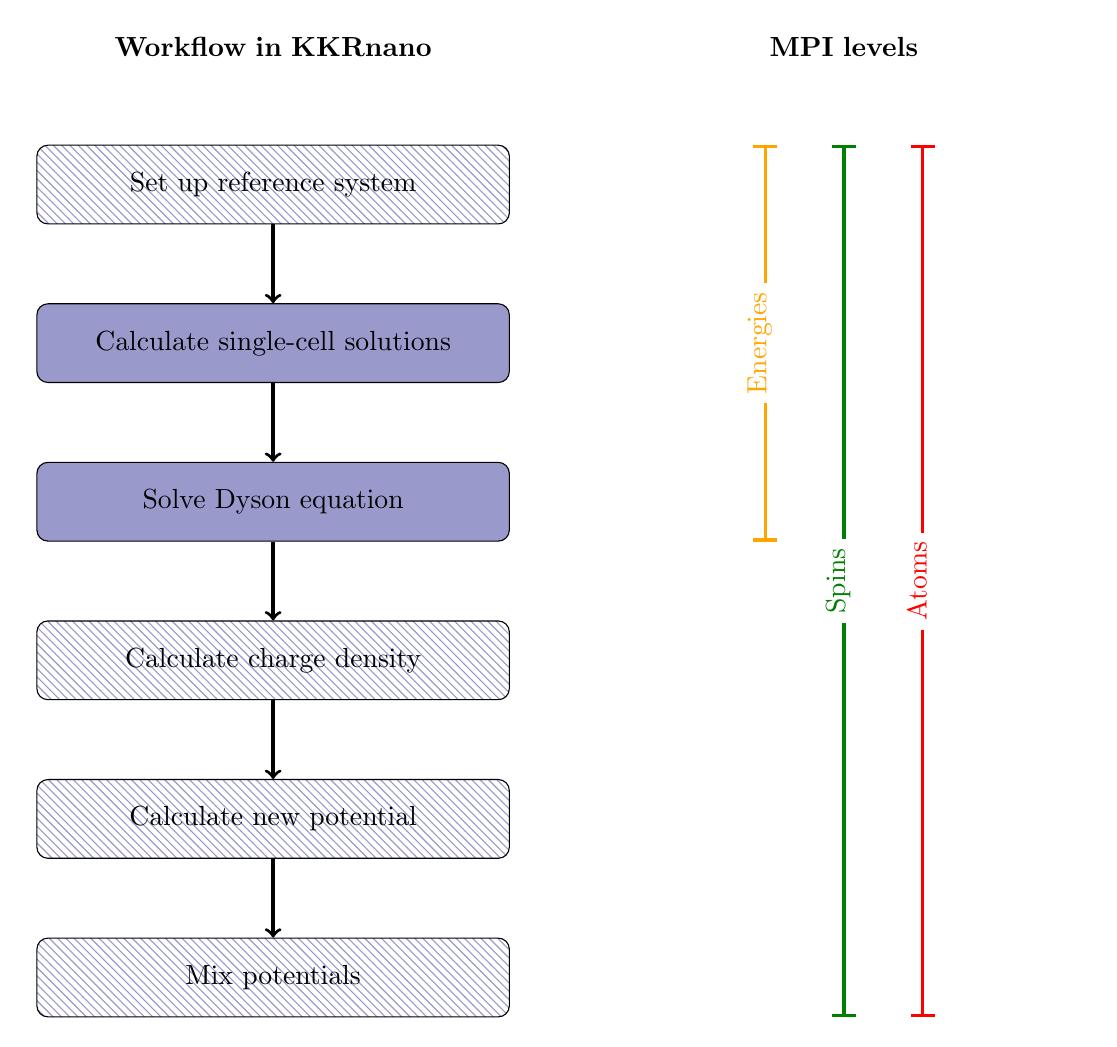
\begin{tikzpicture}[node distance=1cm]
%	\tikzstyle{process} = [rectangle, minimum width=3cm, minimum height=1cm, text centered, draw=black, fill=orange!30]
%	\tikzstyle{decision} = [diamond, minimum width=3cm, minimum height=1cm, text centered, draw=black, fill=green!30]
	\tikzstyle{serial_part} = [rectangle, rounded corners, minimum width=6cm, minimum height=1cm,text centered, draw=black]
	\tikzstyle{omp_part} = [rectangle, rounded corners, minimum width=6cm, minimum height=1cm,text centered, draw=black, fill=NavyBlue!40]
	\tikzstyle{omp_part2} = [rectangle, rounded corners, minimum width=6cm, minimum height=1cm,text centered, draw=black, pattern=north west lines, pattern color=NavyBlue!40]
%	\tikzstyle{io} = [trapezium, trapezium left angle=70, trapezium right angle=110, minimum width=3cm, minimum height=1cm, text centered, draw=black, fill=blue!30]
	\node (title1) [text centered, text width=6cm] {\textbf{Workflow in KKRnano}};
	\node (title2) [text centered, text width=6cm, right=of title1] {\textbf{MPI levels}};
	\node (ref) [omp_part2, below=of title1] {Set up reference system};
	\node (single) [omp_part, below=of ref] {Calculate single-cell solutions};
	\node (dyson) [omp_part, below=of single] {Solve Dyson equation};
	\node (charge) [omp_part2, below=of dyson] {Calculate charge density};
	\node (pot) [omp_part2, below=of charge] {Calculate new potential};
	\node (mix) [omp_part2, below=of pot] {Mix potentials};

\draw [Black, very thick, ->] (ref.south) -- (single.north) ;
\draw [Black, very thick, ->] (single.south) -- (dyson.north) ;
\draw [Black, very thick, ->] (dyson.south) -- (charge.north) ;
\draw [Black, very thick, ->] (charge.south) -- (pot.north) ;
\draw [Black, very thick, ->] (pot.south) -- (mix.north) ;
	% MPI regions
	\def\AtomShift{8.25cm}
	\def\SpinShift{7.25cm}
	\def\EnergyShift{6.25cm}
	 \draw [Red, very thick, |-|] ([xshift=\AtomShift]ref.north) -- ([xshift=\AtomShift]mix.south) node [midway, rotate=90, fill=white, yshift=2pt] {Atoms} ;
	 \draw [Green, very thick, |-|] ([xshift=\SpinShift]ref.north) -- ([xshift=\SpinShift]mix.south) node [midway, rotate=90, fill=white, yshift=2pt] {Spins} ;
	 \draw [Orange, very thick, |-|] ([xshift=\EnergyShift]ref.north) -- ([xshift=\EnergyShift]dyson.south) node [midway, rotate=90, fill=white, yshift=2pt] {Energies} ;
	%	\draw[->, to path={-| (\tikztotarget)}]
%	  (ref) edge (mix) edge;
%	\node (dec1) [decision, below of=pro1, yshift=-0.5cm] {Decision 1};
%	\node (pro2a) [process, below of=dec1, yshift=-0.5cm] {Process 2a};
%	\node (pro2b) [process, right of=dec1, xshift=2cm] {Process 2b};
%	\node (out1) [io, below of=pro2a] {Output};
%	\node (stop) [startstop, below of=out1] {Stop};
\end{tikzpicture}
\caption{Schematic representation of MPI and OpenMP parallelization in KKRnano.
The most important steps in the KKR workflow are depicted on the left side and the
three MPI regions over atoms, spins and energy points are indicated on the right side.
Parts filled with blue comprise routines
where OpenMP is used and where this can be of high importance to the overall performance 
while in the striped blue parts
OpenMP is used but is less significant.
Published with kind permission of © Marcel Bornemann 2018. All Rights Reserved.
}
\label{fig:kkrnano_parallel}
\end{figure}

\subsubsection*{MPI parallelization over atoms}

The most crucial MPI level in KKRnano is the one for atoms since application scenarios for KKRnano
involve the treatment of a few thousand atoms and the KKR formalism allows us to solve the
multiple-scattering problem locally for each atom, if the Green functions of the reference system and
the $\Delta t$-matrices of the other scattering centers are provided (see \cref{eq:dyson_eq}).
In practice, one MPI task handles 1-16 atoms.
The reference Green functions are calculated by each task
for the atoms it is responsible for and are then sent to other tasks that require them. 
The reference t-matrices for the atoms inside the respective reference cluster are not communicated 
but calculated by each task individually as it takes less time to re-compute them compared to communicating them.
In any case, the $\Delta t$-matrices of the actual systems need to be communicated.
After the necessary information is distributed, the Dyson equation can be solved independently by each task.
The calculation of the local charge density can also be conducted locally since only the diagonal
$nn$-elements are needed for this.
In order to subsequently obtain the potential from the local charge moments via the Poisson equation,
the moments must be shared with all other atom tasks by means of all-to-all communication.
The communcation pattern prevents a good scaling behaviour in this part of the code and we currently develop
an implementation which works without all-to-all communication.

\subsubsection*{MPI parallelization over spin channels}

If the system of interest is a collinear magnet, the two spin channels can be handled by two distinct
MPI tasks since the
magnetic Kohn-Sham equations are separable.
Due to the relatively small additional MPI communication effort,
this yields an almost ideal speed-up by a factor of 2 in the important
multiple-scattering part of the calculation.
It should be noted that in the non-collinear KKR formalism such a 
separation of spin channels is no longer possible because 
there is intermixing and all operations involving the
$\Delta t$-matrices and Green functions
need to be performed in full spin space, i.e., $\{\uparrow \uparrow, \uparrow \downarrow,
\downarrow \uparrow, \downarrow \downarrow \}$.
Thus, the spin parallelization level can only be used in connection with
a collinear calculation.


\subsubsection*{MPI parallelization over energy points}

The requirement to calculate the Green function at different energy points offers another possibility to
introduce a parallel level since the values of the Green function $G(\epsilon_i)$ at energy points $\epsilon_i$
can be obtained in parallel.
After the values are obtained, the results must be distributed among the processes within
the energy parallelization level to recover the full Green function at all energy points.
Assigning one MPI task to each energy point is not a promising concept because
of the significantly different runtimes per energy point. Especially the points closest to the
Fermi level 
need more TFQMR iterations.
Therefore, the energy points are split into three different groups and each group is taken care of by
one MPI task.
In the first iteration of the self-consistency cycle the points are equally distributed to all
groups. At the end of the first iteration the points are regrouped depending on how much time the iteration took
for each point. The aim is to find a grouping for which all groups of energy points are converged at
a similar time so that idling is avoided. This is also referred to as \textit{dynamical load-balancing}.
A correct load-balancing is of outmost importance to the effectiveness of this MPI level since
all tasks need to have finished before the program can move on to the solution of the electrostatic problem,
i.e., the Poisson equation.
Due to the challenge that load-balancing can pose, parallelization over energy points should only be used, 
if plenty of processor cores
ought to be utilized and the Poisson solver is well-scaling.

\subsubsection*{OpenMP parallelization}

KKRnano can be compiled either with or without support for OpenMP.
If it is enabled,
loops primarily in the TFQMR solver but also in the routines that calculate the single-cell
solutions are executed using parallel threads. 
This is particularly useful on architectures that support simultaneous multithreading (SMT).
However, we try to use BLAS (Basic Linear Algebra Subprograms) library routines for arithmetic
operations, e.g., matrix-matrix multiplications, throughout our code. BLAS libraries usually
have their own built-in SMT support.
Therefore, the available SMT threads must be partitioned between the explicit OpenMP 
parallel regions in the code and the implicit parallelization of the BLAS library.
Here, the optimal partitioning is highly architecture-dependent and a general recommendation cannot
be given. On Hazel Hen the best performance is achieved, when all threads are used by the BLAS library.


\subsubsection*{Multiple Atoms per MPI Task}

Assigning multiple atoms to one MPI task is beneficial, if very large systems are
supposed to be calculated on a comparatively small allocation of compute nodes.
KKRnano can treat multiple atoms per atomic MPI task by using the following algebraic scheme: 
We rewrite the Dyson equation (see \cref{eq:dyson_eq} and \cref{eq:axb}) with indices so that it reads
\beq
\sum_{\mu} \sum_{L'} A^{\nu \mu}_{LL'} X^{\mu}_{L'L''} = b_{L'L''},
\label{eq:dyson2}
\eeq
where $\nu$ and $\mu$ indicate atomic indices and $L$, $L'$ and $L''$ denote
the appropriate expansion in angular momentum components.
In order to describe the dimensions of the constituents of the equation above, we
declare the following parameters:
$N_{\text{cl}}$ is the number of atoms in the reference cluster that defines the reference Green function.
$N_{\text{tr}}$ is the number of atoms in the truncation cluster. Only interactions with atoms that lay 
within the truncation cluster of an atom are considered. This is essential to achieve
the linear-scaling of the multiple-scattering problem. 
All quantities are expanded in spherical harmonics up to $l_{\text{max}}$, which is usually fixed to
$l_{\text{max}}=3$.
With these definitions we return to \cref{eq:dyson2}, where $A$ is of dimension 
$N_{\text{cl}} (l_{\text{max}}+1)^2 \times N_{\text{tr}} (l_{\text{max}}+1)^2$,
$b$ usually has the
negative local $\Delta t$ as diagonal elements
and $X$ has dimension $N_{\text{tr}} (l_{\text{max}}+1)^2 \times (l_{\text{max}}+1)^2$.
$A$ is a matrix of blocks of size ${(l_{\text{max}}+1)}^2 \times {(l_{\text{max}}+1)}^2$,
while $X$ and $b$ are vectors
of such blocks. For more than a single atom per task, $x$ and $b$ can also take a matrix form
with dimension $N_{\text{cl}} (l_{\text{max}}+1)^2 \times N_{\text{loc}} (l_{\text{max}}+1)^2$, where
$N_{\text{loc}}$ is the number of atoms treated by one MPI task of the atom parallelization level.
The corresponding linear system of equations reads
\beq
\label{eq:dyson_equation_lap_multi}
\sum_{\mu} \sum_{L'} A^{\nu \mu}_{LL'} X^{\mu \gamma}_{L'L''} = b^{\gamma}_{L'L''},
\eeq
where an additional index $\gamma$ is introduced that runs over $N_{\text{loc}}$. 


\section{Performance of KKRnano on Hazel Hen}
\label{sec:performance}

In this section we present performance results of KKRnano that were obtained on Hazel Hen.
A runtime analysis of the parts that are related to the specific physical problems is given
which is followed by an overview of how much time is spent in distinct
classes of routines, e.g., library calls and MPI communication.
The weak-scaling benchmarks on Hazel Hen are performed for B20-\ce{MnGe} 
with the magnetic moments being treated as
non-collinear.
For this, KKRnano is compiled with the Intel Fortran compiler
with optimization level O2 and linked to the Intel Math Kernel (MKL) library which handles all BLAS calls.
The runs are conducted with a task distribution of 24 MPI processes per node. The OpenMP threads 
are reserved for the multi-threaded MKL library.
We choose two atomic supercells containing 1728 and 13824 atoms 
and perform one self-consistency step for each system.
We solely activate the MPI parallelization level over atoms and do not use the ones over spins and energies.
Then, 72 and 576  nodes
are needed for the two benchmark calculations, since each MPI task is assigned to one atom. 
Each MPI process reads four shared binary direct-access
files before commencing the self-consistency step.
Two of them are index-files of the size of a few hundred kByte while the other two can grow with system size
up to several GByte. The combined size of all files that are 
read in is roughly $N$ $\times$ 0.5 MBytes, where $N$ is the number of atoms. 
After the single self-consistency step 
the potential is written out. 
This and the read-in of the four files mentioned above accounts for most of the time spent in I/O.
\begin{figure}[htb]
\begin{center}
 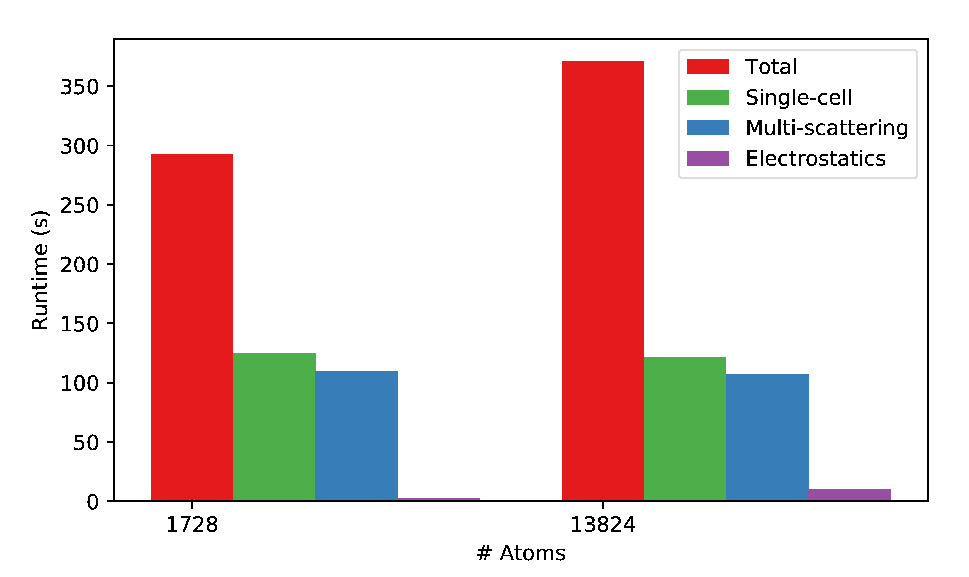
\includegraphics[width=1.0\textwidth]{Figures/MnGe_benchmarks.eps}
\end{center}
	\caption{Runtime of a single DFT self-consistency step
	for different B20-\ce{MnGe} supercell sizes with KKRnano. 
	The total runtime and the individual runtimes for the single-cell solver,
	the multiple-scattering solver and the electrostatics solver are given.
	Published with kind permission of © Marcel Bornemann 2018. All Rights Reserved.
	}
\label{fig:MnGe_6x6x6_benchmark}
\end{figure}
\Cref{fig:MnGe_6x6x6_benchmark}
shows the total runtimes of a single self-consistency iteration and how much time is spent
on solving the individual physical problems for the two supercells containing 1728 and 13824 atoms, respectively.
The remaining time
can be mainly attributed to Fortran direct-access I/O which does not scale well on a Lustre file system.
The observation of an increase in total runtime for larger systems is a strong hint to this as the amount of
file accesses is proportional to the number of MPI processes.
The implementation of a more suitable I/O library (e.g., MPI I/O or SIONlib) is likely to solve this issue.
The multiple-scattering solver, i.e., the TFQMR solver, 
and the solution of the relativistic single-cell problem are
expected to account for most of the computational work in KKRnano which 
is why linear scaling is of particular importance in these parts of the code.
Our results show that both parts scale indeed linearly, i.e., the runtime stays constant as long as
the ratio of CPU cores to atoms remains constant.
Furthermore, it should be noted that the walltime that is needed for a single self-consistency step of a system
that includes 1728 atoms
takes less than five minutes which is a good value, especially when considering that
the magnetic moments are allowed to be non-collinear.
In the KKR formalism, the electron density and the potential are connected via the Poisson equation. 
For very large systems the Poisson solver contributes considerably
to the overall runtime \cite{brommel_juqueen_2017}.
This is expected since the algorithm used in KKRnano scales
quadratically with the number of atoms. Its impact when mid-sized systems are investigated is negligible. 
However, there are ideas on how to restructure the Poisson solver towards a more favorable scaling behavior.
This is planned for the near future.

Next, we conduct a performance analysis on the level of individual routines.
The Cray Performance Tools package provides a helpful collection of tools to gather data for this purpose.
It allows to sample the time that is spent within each routine and can therefore give a good
impression of which routines are performance-critical and should be considered for further optimization.
\begin{figure}[htb]
\begin{center}
 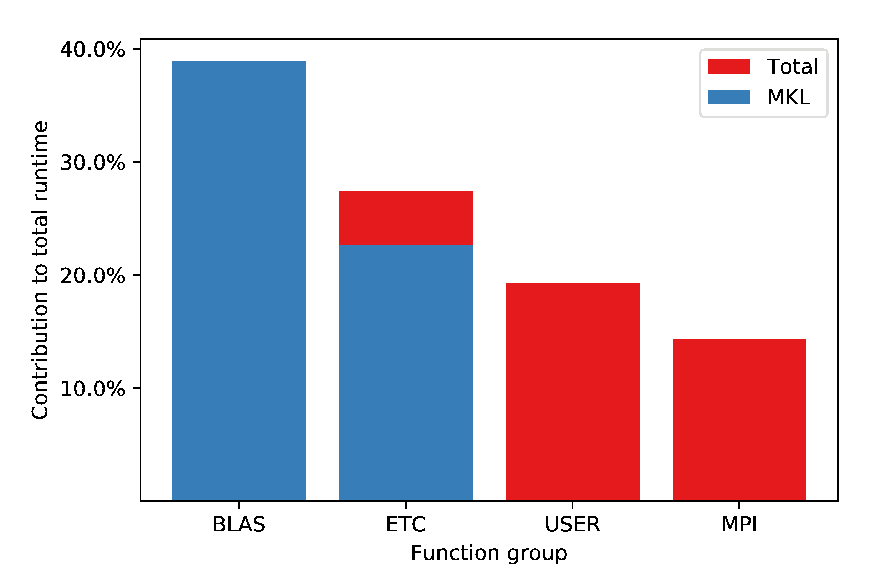
\includegraphics[width=0.8\textwidth]{Figures/MnGe_6x6x6_crayreport.eps}
\end{center}
	\caption{Runtime results from Cray Performance Measurement 
	Tool for a single KKRnano self-consistency step 
	for a 6x6x6 supercell of B20-\ce{MnGe} (1728 atoms). 72 Hazel Hen nodes are used with 1728 MPI processes.
	The runtimes are divided into four subgroups which are described in the text.
	The fraction of the total runtime in each subgroup that is spent in
	routines of Intel's highly-optimized MKL library is highlighted in blue.
	Published with kind permission of © Marcel Bornemann 2018. All Rights Reserved.
	}
\label{fig:MnGe_6x6x6_crayreport}
\end{figure}
\Cref{fig:MnGe_6x6x6_crayreport} shows the sampling results for a 6x6x6 supercell calculation
of B20-\ce{MnGe} using 1728 MPI tasks on 72 nodes.
The routines are grouped according to their origin. The \textit{BLAS} group comprises the kernels of
library-based linear algebra operations. 
All external routines for which no source file was given at compile time are subsumed
in \textit{ETC}. Such routines are e.g. Fortran I/O routines and MKL helper routines
that are indispensable for BLAS but are not directly related
to the MKL kernel.
The \textit{USER} group accounts for all routines from the KKRnano source code, i.e., our self-written routines.
Finally, \textit{MPI} contains all the routines that are needed for communication and synchronization
between the MPI tasks. 
Performing linear algebra operations accounts for almost 40 \% of the total runtime. Prior tests have shown that
Intel's MKL outperforms Cray's LibSci and therefore KKRnano is linked to the former.
The routines that fall into the \textit{ETC} category consume 28 \% of the total runtime. 
The MKL routines dominate this group and it can be stated that the ratio of MKL in the total runtime is 62 \%.
This is a remarkable value as it indicates that more than half of the walltime is spent in routines
that are already highly optimized.
The only group of routines that can benefit from source code tuning is the \textit{USER} group.
However, a hypothetical performance improvement by a factor of two would lead to
an overall performance increase of merely 10 \% as the share of this group in the total runtime is only 20 \%.
MPI routines are not crucial to performance as they amount to only 15 \% of the total
computational effort.


\section{Conclusions}
In this report we introduced an extended Korringa-Kohn-Rostoker method as the foundation of our large-scale
Density Functional Theory application KKRnano. 
Consecutively, we presented results that were obtained on Hazel Hen 
by applying KKRnano to the material B20-\ce{MnGe}.
Those results are promising and suggest further investigation
of complex magnetic textures in this particular compound.
The high-clocked Intel Xeon processors of Hazel Hen
make a single DFT self-consistency step for a supercell of 1728 atoms feasible within 
less than five minutes and hence allows one
to obtain results in a timely manner.

During the
\textit{Optimization of Scaling and Node-level Performance on Hazel Hen} workshop at HLRS in 2018 we were
given the chance to further optimize our code and were able to identify a computational bottleneck. 
The performance of KKRnano on Hazel Hen was significantly improved by resolving it. The encountered problem was
connected to unnecessary copying of a large complex-valued array, when the magnetic moments are allowed to be
non-collinear.
All results in \cref{sec:performance} were
obtained with this optimized version.
Further optimization for standard calculations with a few thousand atoms 
is difficult since only 20 \% of the runtime is spent in hand-written code. The remaining 80 \% is spent in
library calls that are already highly tuned. These routines mainly deal with
MKL-BLAS and MPI communication.
%\\
%We conclude with a request with regards to the job scheduling on Hazel Hen:
%For our purposes it would be beneficial, if relatively small jobs with an allocation of
%about 100 nodes 
%were scheduled with higher priority than they currently are.

%
\begin{acknowledgement}
The authors gratefully acknowledge the Gauss Centre for Supercomputing e.V. (www.gauss-centre.eu)
for funding this project by providing computing time through the project GCS-KKRN on the GCS Supercomputer
Hazel Hen at Höchstleistungsrechenzentrum Stuttgart (HLRS).
%The computing time that was provided for this project on Hazel Hen in Stuttgart (project ID 44129) and
%QPACE3 in J\"ulich is gratefully acknowledged.
%If you want to include acknowledgments of assistance and the like at the end of an individual chapter please use the \verb|acknowledgement| environment -- it will automatically render Springer's preferred layout.
\end{acknowledgement}

% Bibliography %%%%%%%%%%%%%%%%%%%%%%%%%%%%%%%%%%%%%%%%%%%%%%%%%%%
\bibliographystyle{spphys}
\bibliography{references}


\end{document}
